Działanie lasów losowych polega na klasyfikacji za pomocą grupy drzew decyzyjnych. Parametrem, który odpowiada za finalną decyzję jest średnia, gdy przewidywana jest wartość liczbowa lub wynik głosowania dla analizowanej przynależności do klasy. Każde z drzew w lasie losowym jest tworzone w oparciu o próbę, powstałą przez wylosowanie N obiektów ze zbioru uczącego. W każdym węźle danego drzewa podział jest dokonywany na podstawie części losowo wybranych cech, których liczba jest zazwyczaj mniejsza od liczby wszystkich cech. Ma to pozwolić na uzyskanie jak największej niezależności poszczególnych węzłów, czyli zmniejszenie wariancji modelu.
Błąd klasyfikacji może być szacowany na podstawie obiektów nie włączonych do próby.

Implementacja algorytmu lasu losowego została wykorzystana przez pakiet \textit{RandomForest}. Przy pierwotnym budowaniu lasu losowego wzięto pod uwagę trzy parametry takie jak:
\begin{itemize}
    \item ilość drzew (\textit{ntree} = {1, 10,50,100,300,500})
    \item głębokość pojedynczego drzewa (\textit{maxnodes} = {3,10,20,50})
    \item ilość atrybutów rozpatrywana przy tworzeniu węzła (\textit{mtry} = {1,2,3,4,5,6,7,8,9,10})
    \item losowanie próbek do modelu ze zwracaniem i bez (\textit{replace} = {TRUE/FALSE})
\end{itemize}
Do zbadania 240 modelów z wymienionymi parametrami użyto funkcji \textit{train}. 
Funkcja \textit{train} zwraca dwie ważne wartości: dokładność modelu (Accuracy) oraz współczynnik Kappa. Dokładność modelu to nic innego jak ilość poprawnie predykowanych próbek do ilości wszystkich badanych próbek. Współczynnik Kappa parametr, który zawiera informacje o odtwarzalności lub powtarzalności pomiaru zmiennej w różnych warunkach. 

Uzyskane wyniki są przedstawione na rys. \ref{fig:all_Dalc}:

\begin{figure}[h]
 \centering 
 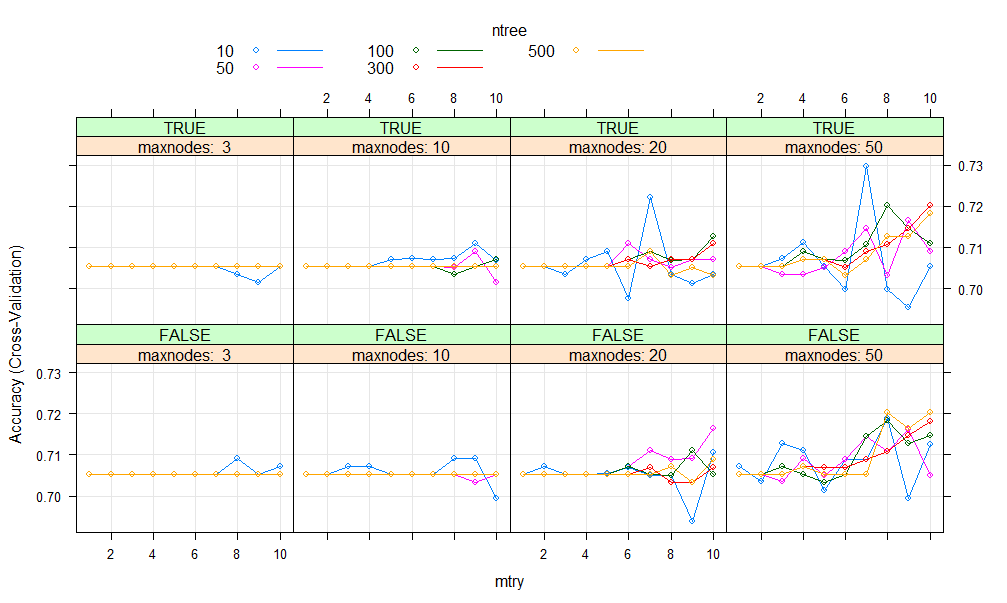
\includegraphics[scale=0.60]{tex/customD_vol4.png}
 \caption{Dokładność predykcji modelu dla klasy spożywającej alkohol w tygodniu (\textbf{Dalc}) w zależności od różnych kombinacji parametrów.}
 \label{fig:all_Dalc}
\end{figure}

    % #mtry ntree maxnodes replace
% #248    7    10       50    TRUE

Na podstawie przeprowadzonych badań dla spożywania alkoholu w tygodniu (\textbf{Dalc}) okazuje się, że najlepszy jest w tym przypadku model zbudowany z zaledwie 10 drzew oraz 7 atrybutów wykorzystywanych do wyboru podziału na każdym poziomie, maksymalnie 50 węzłów w drzewie oraz wykorzystywania losowania ze zwracaniem. W tabeli \ref{tab:best_Dalc_forest} zestawiono wyniki uzyskane przez ten model.
Całkowita wartość błędu \textbf{out-of-bag} to 29.62\%, co oznacza że dokładnie 70.38\% próbek zostało poprawnie sklasyfikowanych. Warto jednak zwrócić uwagę, że na ten wynik składa się głównie poprawna klasyfikacja dla najliczniejszej klasy 1. Dla pozostałych klas model prawie zawsze się mylił.

\begin{table}[h]
\centering
\caption{Wyniki predykcji dla najlepszego modelu lasu losowego \textbf{Dalc}}
 \label{tab:best_Dalc_forest}
\begin{tabular}{|c|c|c|c|c|c|c|}
\hline
\multirow{}{}{\textbf{\begin{tabular}[c]{@{}c@{}}klasa\\ prawdziwa\end{tabular}}} & \multicolumn{5}{c|}{\textbf{predykcja}}                                & \multirow{}{}{\textbf{błąd klasy [\%]}} \\ \cline{2-6}
                            & \textbf{1} & \textbf{2} & \textbf{3} & \textbf{4} & \textbf{5} &                                      \\ \hline
\textbf{1}                  & 343        & 14         & 5          & 0          & 2          & 5,77                           \\ \hline
\textbf{2}                  & 68         & 19         & 6          & 0          & 0          & 79,57                           \\ \hline
\textbf{3}                  & 22         & 10         & 3          & 0          & 2          & 91,89                           \\ \hline
\textbf{4}                  & 5          & 3          & 2          & 0          & 1          & 100                            \\ \hline
\textbf{5}                  & 10         & 0          & 3          & 0          & 1          & 92,86                          \\ \hline
\end{tabular}
\end{table}



\begin{figure}[h]
     \centering 
     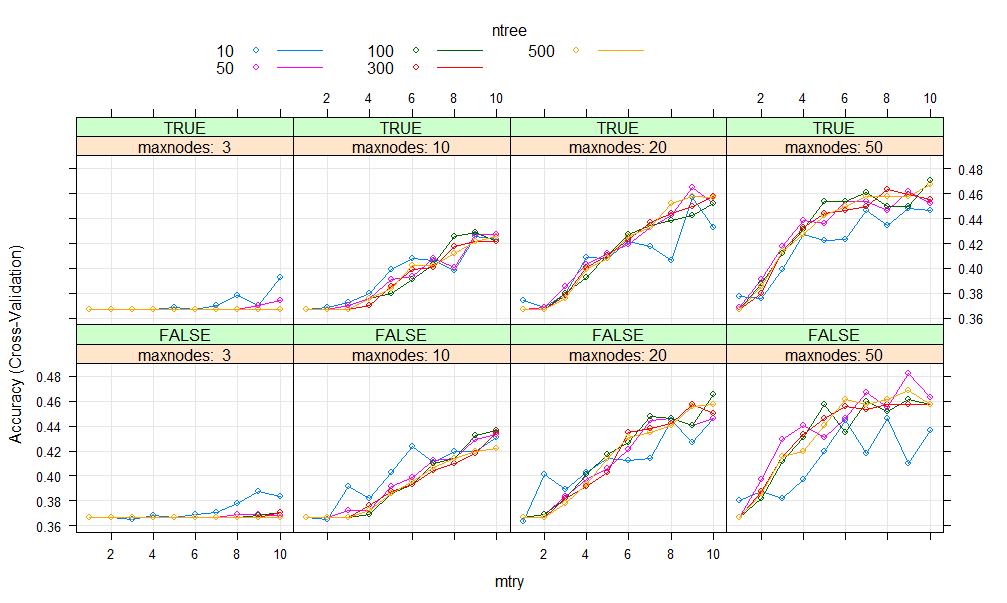
\includegraphics[scale=0.60]{tex/customW_vol4.png}
     \caption{Dokładność predykcji modelu dla klasy spożywającej alkohol w weekend (\textbf{Walc}) w zależności od różnych kombinacji parametrów.}
     \label{fig:all_Walc}
\end{figure}


% plot(custom_W)
% #     mtry ntree maxnodes replace
% # 335    9    50       50   FALSE

Na podstawie przeprowadzonych badań dla spożywania alkoholu w weekend (\textbf{Walc}) wyznaczono jako najlepszy model ten zbudowany z 50 drzew oraz 9 atrybutów wykorzystywanych do  budowania podziału oraz maksymalnie 50 węzłów w drzewie oraz niewykorzystywania losowania ze zwracaniem (rys. \ref{fig:all_Walc}).
 
 \begin{table}[h!]
 \centering
 \caption{Wyniki predykcji dla najlepszego modelu lasu losowego \textbf{Walc}}
 \label{tab:best_Walc_forest}
\begin{tabular}{|c|c|c|c|c|c|c|}
\hline
\multirow{}{}{\textbf{\begin{tabular}[c]{@{}c@{}}klasa\\ prawdziwa\end{tabular}}} & \multicolumn{5}{c|}{\textbf{ predykcja}}                                & \multirow{}{}{\textbf{błąd klasy [\%]}} \\ \cline{2-6}
                            & \textbf{1} & \textbf{2} & \textbf{3} & \textbf{4} & \textbf{5} &                                      \\ \hline
\textbf{1}                  & 179        & 7          & 7          & 0          & 1          & 7,73                           \\ \hline
\textbf{2}                  & 88         & 13         & 15         & 7          & 0          & 89,43                         \\ \hline
\textbf{3}                  & 50         & 18         & 12         & 22         & 1          & 88,43                          \\ \hline
\textbf{4}                  & 25         & 9          & 21         & 22         & 1          & 71,79                           \\ \hline
\textbf{5}                  & 7          & 3          & 5          & 8          & 8          & 74,19                          \\ \hline
\end{tabular}
\end{table}
Łączna wartość błędu \textbf{out-of-bag} to 55.77\%, co oznacza że dokładnie 44.23\% próbek zostało poprawnie sklasyfikowanych. W tym przypadku błąd jest znacznie większy niż dla opisującej spożycie alkoholu w ciągu tygodnia, wynika to liczniejszej reprezentacji poszczególnych klas, dla których błędy wynoszą 70-90\%. Klasa 1 wciąż klasyfikowana jest małym błędem.
\subsection{Wpływ zmiennych na jakość modelu}
W celu całkowitego wyczerpania tematu - sprawdzono jak wygląda predykcja modelu przy zachowaniu 2 stałych parametrów a zmieniając trzeci. Dwa ustalone parametry były dobierane na podstawie wcześniejszych eksperymentów. Liczba drzew została ustalona na 100, tak aby wariancja pojedynczego drzewa nie wpływała znacząco wynik skuteczności. Założono, że maksymalna głębokość pojedynczego drzewa będzie wynosiła 50, a ilość zmiennych analizowanych przy pojedynczym podziale będzie równa 7. W celu uzyskania wykresów pudełkowych każdy typ modelu został utworzony 50 razy.

\begin{figure}[h]
     \centering 
     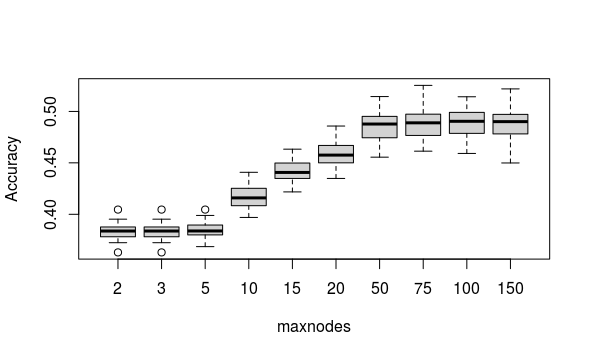
\includegraphics[scale=0.80]{tex/W_maxnodes.png}
     \caption{Zależność dokładności od maksymalnej ilości węzłów dla mtry = 7, ntree = 100: \textbf{Walc}}
     \label{fig:W_maxnodes}
\end{figure}
\begin{figure}[t]
     \centering 
     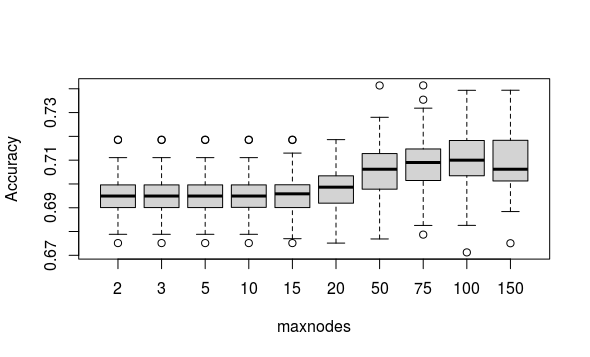
\includegraphics[scale=0.80]{tex/D_nodes.png}
     \caption{Zależność dokładności od maksymalnej ilości węzłów dla mtry = 7, ntree = 100: \textbf{Dalc}}
      \label{fig:D_maxnodes}
\end{figure}
\FloatBarrier
Zwiększając ilość możliwych poziomów w pojedynczym drzewie zwiększana jest dokładność modelu. Pojedyncze drzewo z tak późno zastosowanym kryterium stopu, zastosowane samodzielnie jako klasyfikator zostałoby najprawdopodobniej uznane jako nadmiernie dopasowane. Dzięki temu zabiegowi dla elementów lasu możliwe jest uzyskanie większego zróżnicowania drzew, a w wyniku tego model zbiorowy cechuje większa skuteczność klasyfikacji. Większy wpływ tego zjawiska widoczny jest dla danych dotyczących spożycia alkoholu w weekend \textbf{Walc} (rys. \ref{fig:W_maxnodes}), gdzie rozkład klas jest bardziej równomierny.
\FloatBarrier
\begin{figure}[h]
     \centering 
     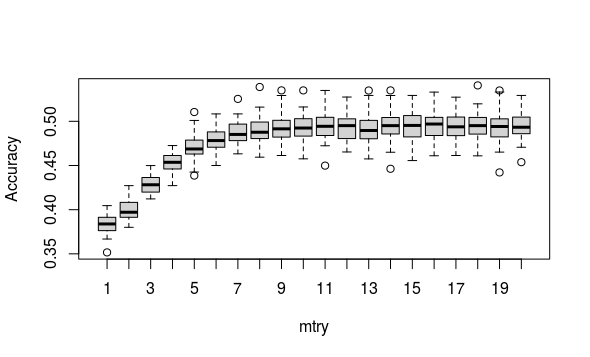
\includegraphics[scale=0.80]{tex/W_mtry.png}
      \caption{Zależność dokładności od mtry dla maxnodes = 50, ntree = 100: \textbf{Walc}}
      \label{fig:W_mtry}
\end{figure}
\begin{figure}[t]
     \centering 
     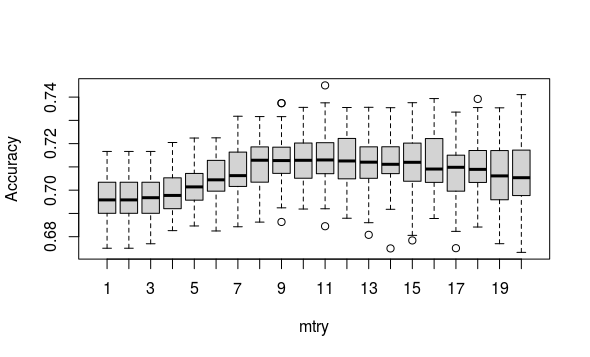
\includegraphics[scale=0.80]{tex/D_mtry.png}
     \caption{Zależność dokładności od mtry dla maxnodes = 50, ntree = 100: \textbf{Dalc}}
     \label{fig:D_mtry}
\end{figure}
\FloatBarrier
Wybór podziału w każdym węźle wykonywany jest na podstawie analizy losowego podzbioru atrybutów. Zwiększając rozmiar tego podzbioru można poprawić jakość klasyfikacji. Stosowana często wartość pierwiastka z liczby atrybutów (w tym przypadku liczba atrybutów to 32, czyli wartość \textit{mtry} powinna wynosić 5--6) znajduje pewne uzasadnienie, pozwala uzyskać lepsze wyniki niż w przypadku zupełnie losowego wyboru. Na każdym poziomie pula analizowanych atrybutów jest inna, co wpływa na większe zróżnicowanie drzew. Na podstawie rys. \ref{fig:D_mtry} można zauważyć, że zbyt duża ilość atrybutów nieznacznie pogarsza jakość klasyfikacji. Prawdopodobnie drzewa stały się do siebie zbyt podobne.
\FloatBarrier
\begin{figure}[h]
     \centering 
     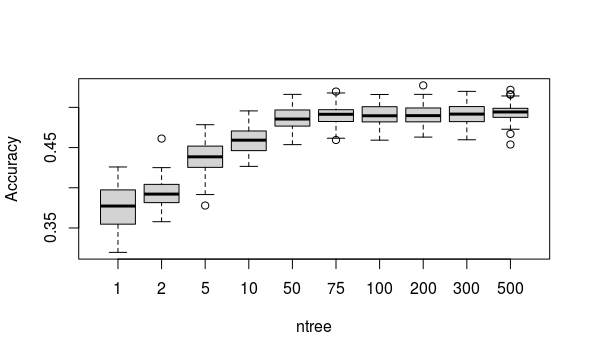
\includegraphics[scale=0.80]{tex/W_ntree.png}
      \caption{Zależność dokładności od ilości drzew dla mtry = 7, maxnodes = 50: \textbf{Walc}}
       \label{fig:W_ntree}
\end{figure}
\begin{figure}[h]
     \centering 
     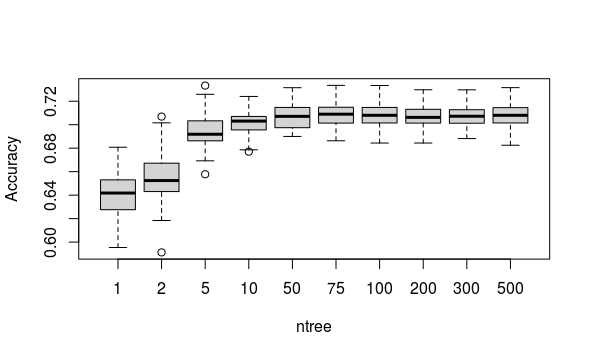
\includegraphics[scale=0.80]{tex/D_ntree.png}
     \caption{Zależność dokładności od ilości drzew dla mtry = 7, maxnodes = 50: \textbf{Dalc}}
     \label{fig:D_ntree}
\end{figure}
\FloatBarrier
Porównując pojedyncze drzewo z modelem zbiorowym obserwowana jest znacząca poprawa dokładności klasyfikacji. Wystarczająco wiele (w tym przypadku już ok. 50) drzew pozwala poprawić jakość i rozrzut predykcji.